\documentclass{article}

\usepackage[utf8]{inputenc}

\usepackage{amsmath}

\usepackage{scrextend}

\usepackage{geometry}
\geometry{
	a4paper,
	total={170mm,257mm},
	left=20mm,
	top=20mm,
}

\usepackage{graphicx}
\usepackage[portuguese]{babel}
\usepackage{subfig}


\usepackage{listings}
\usepackage{xcolor}

\definecolor{codegreen}{rgb}{0,0.6,0}
\definecolor{codegray}{rgb}{0.5,0.5,0.5}
\definecolor{codepurple}{rgb}{0.58,0,0.82}
\definecolor{backcolour}{rgb}{0.95,0.95,0.92}

\lstdefinestyle{mystyle}{
	backgroundcolor=\color{backcolour},   
	commentstyle=\color{codegreen},
	keywordstyle=\color{magenta},
	numberstyle=\tiny\color{codegray},
	stringstyle=\color{codepurple},
	basicstyle=\ttfamily\footnotesize,
	breakatwhitespace=false,         
	breaklines=true,                 
	captionpos=b,                    
	keepspaces=true,                 
	numbers=left,                    
	numbersep=5pt,                  
	showspaces=false,                
	showstringspaces=false,
	showtabs=false,                  
	tabsize=2
}

\lstset{style=mystyle}

%\usepackage{indentfirst}
\setlength{\parindent}{1.5cm}% too much in my eyes delete this
% line and use the default ...


\title{
	Identificando transições abruptas em vídeos (trabalho 3) \\
	\Large Introdução ao Processamento de Imagem Digital \\
	Randerson A. Lemos (103897)
	2022-1S
}

\date{\vspace{-5ex}}

\begin{document}
  \pagenumbering{gobble}
  \maketitle

%
%%
\section{Introdução}
Vídeos são compostos por quadros de mesma dimensão organizados temporalmente. Esses quadros, ao serem apresentados sequencialmente (no contexto do vídeo), podem apresentar transições suaves ou abruptas. Quando presentes, as transições abruptas entre quadros podem indicar uma sequência significativamente nova de conteúdo no vídeo e, por isso, tais transições, quando identificadas, podem ser utilizadas como material de resumo do próprio vídeo. Neste trabalho, utilizaremos quatro técnicas capazes de identificar transições abruptas entre quadros de um vídeo de acordo com certas métricas de distância. As técnicas utilizadas são: \textbf{diferenças entre pixels}; \textbf{diferenças entre blocos}; \textbf{diferenças entre histogramas}; e \textbf{diferenças entre mapas de bordas}.

\subsection{Diferenças entre pixels}
Aqui, para que dois quadros consecutivos sejam considerados diferentes é feita uma contagem do número de par de pixels (um de cada quadro) que são diferentes de acordo com uma tolerância $T_1$. Se essa contagem for superior a um limiar $T_2$, os quadros comparados são considerados diferentes e a transição entre eles entendida como abrupta. Tanto a tolerância $T_1$ quanto o limiar $T_2$ são parâmetros definidos pelo usuário e apresentam valores ótimos dependentes das características de cada vídeo analisado. Para o calculo da diferença entre pixels, cujo valor resultante é utilizado na comparação com a tolerância $T_1$, utiliza-se a norma 1, isto é, a diferença absoluta entre os níveis de cinza do par de pixels analisados dos quadros consecutivos.


\subsection{Diferenças entre blocos}
Na diferenças entre blocos é necessário subdividir os quadros consecutivos em blocos (cada quadro com seu conjunto de blocos). Feito isso, os pares de blocos correspondentes entre os quadros consecutivos são comparados e, de acordo com uma tolerância $T_1$, são ou não considerados diferentes. O número de pares de blocos entre quadros consecutivos considerados diferentes é comparado a um limiar $T_2$ e, caso esse número seja superior a tal limiar, o quadros são considerados diferentes. O blocos que subdividem os quadros possuem ou dimensão de $8x8$ ou de $16x16$. Tanto a tolerância $T_1$ quando o limiar $T_2$ são definidos pelo usuário e seus valores ótimos são dependentes das características de cada vídeo analisado.


\subsection{Diferenças entre histogramas}
Diferente das anteriores, nesta abordagem utilizaremos os histogramas dos quadros consecutivos, e não os valores dos pixels em si, como fonte para realização das comparações e, consequentemente, determinação de transições abruptas ou não entre tais quadros. A diferença $D_i$ entre histogramas de quadros consecutivos $i$ e $i+1$ de uma vídeo é calculada como
\[
D_i = \sum_{j=1}^{B} |H_i(j) - H_{i+1}(j)|,
\]
em que $B$ denota o número total de \textit{bins} no histograma e $H_i(j)$ é o valor do histograma para o i-ésimo quadro no nível $j$. Para avaliar se os quadros consecutivos são diferentes o suficiente para considerar que a transição correspondente seja abrupta, um limiar $T$ é calculado a partir do conjunto de todas as diferenças $D_i$ calculadas. Em posse da média $\mu$ e do desvio padrão $\sigma$ das diferenças $D_i$ o limiar $T$ é obtido pela equação
\[
T = \mu + \alpha\sigma,
\]
em que $\alpha$ é definido pelo usuário. Ao parâmetro $alpha$ é atribuído valores típicos entre $3$ e $6$.¨


\subsection{Diferenças entre bordas}
Na diferenças entre bordas, utiliza-se o mapa de bordas dos quadros consecutivos como fonte de informação para determinação ou não de uma transição abrupta entre esses quadros. A abordagem adotada para verificação da diferença entre quadros consecutivos foi a contagem do número de pixels das bordas de cada quadro seguida da subtração absoluta desses valores. O número resultante dessa operação é comparado com um limiar $T$. Caso tal número seja superior que esse limiar, os quadros são considerados diferentes e a transição correspondente abrupta. 
%
%%
\section{Solução}
A solução utiliza a linguagem de programação Python e conta com o auxílio do gerenciador de projetos e pacotes Conda. Assumindo que o usuário tenha o Conda instalado em sua máquina, a configuração do projeto pode ser feita pela execução do comando \lstinline{conda env create -f environment.yml} a partir da pasta do projeto \textbf{trab3}. Esse comando cria o ambiente de trabalho \textbf{mc920-trab3} e instala os seguintes módulos: opencv, numpy, scipy, pandas, matplotlib. Finalizada a configuração do ambiente de trabalho em questão, o usuário deve executar o comando \lstinline{source source.sh}\footnote{O comando que configura o ambiente de trabalho mc920-trab3 precisa ser executado apenas um vez. Assim sendo, depois que este ambiente está configurado, o usuário precisa apenas executar o comando \lstinline{source source.sh}} para carregar as variáveis de ambiente adequadas e, assim, poder usar os programas do projeto dentro do próprio ambiente de trabalho recém configurado. 

Dos arquivos presentes na pasta do projeto \textbf{trab3}, destacam-se as pastas \textbf{assets}, \textbf{classes}, \textbf{tex} e o programa \textbf{main.py}. A pasta \textbf{assets} contém vídeos no formato png ou mpg que podem ser utilizadas para a aplicação das técnicas de identificação de transições abruptas implementadas. A pasta \textbf{classes} contém arquivos com as implementações das diferentes técnicas de identificação de transições abruptas em formato de classes. Os arquivos das classes das técnicas são: \textbf{blocksdifferences.py}, \textbf{edgesdifferences.py}, \textbf{histogramdifferences.py}, e \textbf{pixelsdifferences.py}. A pasta \textbf{tex} contém os arquivos Latex deste relatório. O programa \textbf{main.py} contém as implementações necessárias para aplicar as técnicas de identificação de transições abruptas no vídeo de entrada fornecido pelo usuário. Informações pertinentes das implementações serão apresentadas a seguir.


\subsection{Main.py}
O programa \textbf{main.py} é responsável pela aplicação de todas as técnicas consideradas de identificação de transições abruptas entre quadros consecutivos de vídeos. Para ser executado, esse programa precisa receber o parâmetro de entrada \textbf{video\_entrada}:

\begin{itemize}
	\item ao parâmetro \textbf{vídeo\_entrada} deve-se fornecer o nome do arquivo do vídeo a ser utilizado para aplicação das técnicas de identificação de transições abruptas.
\end{itemize}
	
\noindent 
O programa \textbf{main.py} disponibiliza tanto um vídeo no formato $mp4$ dos quadros considerados como pertencentes a transições abruptas como gráficos em formato png da evolução dos valores de distância utilizados para determinação de transição abrupta ou não. Todo esse conteúdo é salvo dentro da pasta \textbf{out} que está localizada dentro da pasta do projeto \textbf{trab3.}


Um exemplo de como executar o programa \textbf{main.py} utilizando os recursos contidos dentro do próprio projeto é: \lstinline{python3 main.py -video_entrada=assets/lisa.mpg}.

O programa \textbf{main.py} executa quatro funções principais, as quais são: \textbf{main\_pixels\_differences( path, stem )}; \textbf{main\_blocks\_differences( path, stem )}; \textbf{main\_histog\_differences( path, stem )}; e \textbf{main\_edges\_differences( path, stem )}. Cada uma dessas funções é responsável por executar a técnica de identificação de transição abrupta associada várias vezes utilizando diferentes combinações de parâmetros de entrada (tolerâncias e limiares). Essas funções também estão encarregas de salvar todo o conteúdo gerado (os vídeos e gráficos) com nomes intuitivos dentro da pasta \textbf{out}. A seguir olharemos para essas funções e, principalmente, para as técnicas de identificação de transições abruptas associadas.

%Sobre a direção de varredura para aplicação das técnicas de meios-tons optou-se por seguir com a direção que percorre a imagem da esquerda para a direita e de cima para baixo (direção \textit{default}) e com a direção da esquerda para direita com alternância e de cima para baixo (direção zig-zag) como ilustrado na imagem da Figura \ref{fig:direcao_varredura}.
%
%\begin{figure}[!htp]%
%	\centering
%	\subfloat[\centering Direção de varredura da esquerda para direita (\textit{default})]{{ 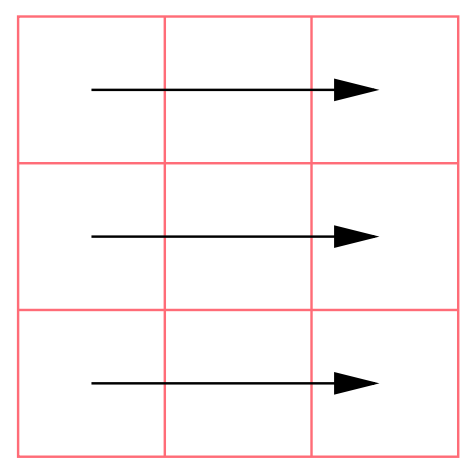
\includegraphics[width=4cm]{varredura.png} }}%
%	\qquad
%	\subfloat[\centering Direção de varredura da esquerda para direita com alternância (zig-zag)]{{ 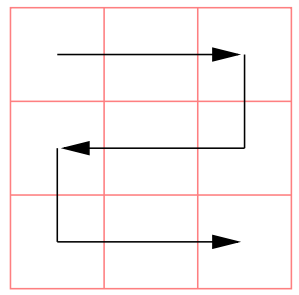
\includegraphics[width=4cm]{varredura_zigzag.png} }}%	
%	\caption{Direção de varredura considerada para aplicação das técnicas de meios-tons (fonte: imagem extraida do documento pdf com as orientações deste trabalho).}%	
%	\label{fig:direcao_varredura}%
%\end{figure}
%
%\noindent
%Essas opções de varredura foram consideras porque a aparência visual das imagens resultantes se mostrou satisfatório, não havendo padrões estranhos que causassem desconforto ao olhar do observador.
%
%Para o processo de aplicação das técnicas de meios-tons em imagens coloridas optou-se por trabalhar no mapa de cores HSV cujas letras são abreviações de \textit{Hue} (matiz), \textit{Saturation} (saturação) e \textit{Value} (valor). Assim, as imagens que, quando carregadas pelo opencv, eram disponibilizadas no mapa de cores BGR tiveram este mapa de cores convertido para o mapa HSV. Já no mapa de cores HSV, apenas o canal V (Value) da imagem (que é o que contém a intensidade luminosa) foi passado para as funções responsáveis pela aplicação das técnicas de meios-tons por difusão de erro. Obtido o canal V em meios-tons, este foi integrado ao esquema HSV original e a nova imagem foi reconvertida para o mapa de cores BGR.
%
%Um dos destaques das implementações realizadas é a classe \textbf{Mask}. Essa classe ficou responsável pelo encapsulamento da lógica de recuperação dos pesos das mascaras das técnicas de meios-tons por difusão de erro bem como das posições nas quais estes pesos devem ser aplicados na imagem original. Dessa maneira, para o usuário, só ficou necessário passar a matriz da mascara da técnica de meio-tom em questão e a posição de referência do posicionamento na mascara do pixel \textbf{f(x,y)} da imagem original. Essa classe foi implementada como um objeto \textbf{iterador} do Python de modo que a obtenção dos pesos bem como da posição de aplicação destes na imagem original era facilmente alcançada dentro de uma estrutura de laço de repetição. Isso tornou bastante conveniente a integração da instancia da classe \textbf{Mask} dentro da função responsável por construir a imagem \textbf{g(x, y)} possuidora dos pixels em meios-tons. A implementação da classe \textbf{Mask} é apresentada a baixo.
%
%\begin{lstlisting}
%class Mask:
%  def __init__(self, mask):
%    self.name = mask.name
%    self.mask = mask.mask
%    self.ref = mask.ref
%
%
%  def __iter__(self):
%    self._r = 0
%    self._c = -1 
%    return self
%
%
%  def __next__(self):
%    mask = self.mask
%    row, col = mask.shape
%    _r = self._r; _c = self._c
%
%    _c += 1
%    if _c == col:
%      _r += 1 
%      _c = _c % col
%
%    while True:
%      if _r < row:
%        val = mask[_r][_c]
%
%        if val:
%          self._r = _r
%          self._c = _c
%          inc = (_r - self.ref[0] , _c - self.ref[1], )
%          return val, inc # retorna o peso a ser multiplicado pelo erro e o incremento
%                          # a ser adicionando no pixel (x,y) da imagem f para difusao
%                          # do erro
%
%        _c += 1
%        if _c == col:
%          _r += 1 
%          _c = _c % col
%
%      else:
%        break
%
%  raise StopIteration
%\end{lstlisting}
%
%Para demais informações acerca das implementações ou algoritmos utilizados, consultar o código fonte. Lá existem comentários que abrangem esse tipo de informação.

%
%%
\section{Resultado}
Os resultados levantados são provenientes da aplicação do programa \textbf{main.py} sobre as imagens apresentadas na Figura \ref{fig:imagem:entrada}. 

%\begin{figure}[!htp]%
%	\centering
%	\subfloat[\centering Vesão colorida da imagem Baboon (original)]{{ 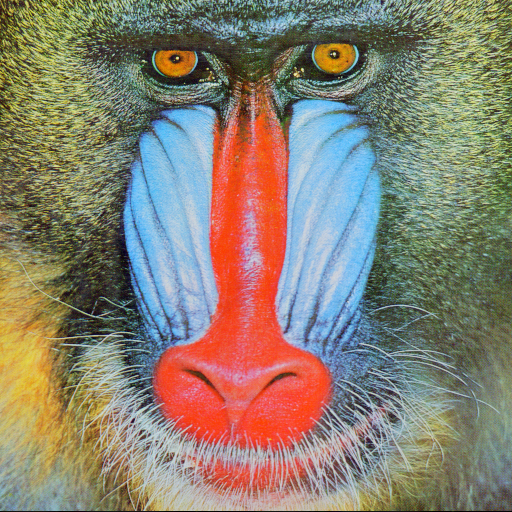
\includegraphics[width=5cm]{../out/cbaboon.png} }}%
%	\qquad
%	\subfloat[\centering Versão em escala de cinza da imagem Baboon (convertida)]{{ 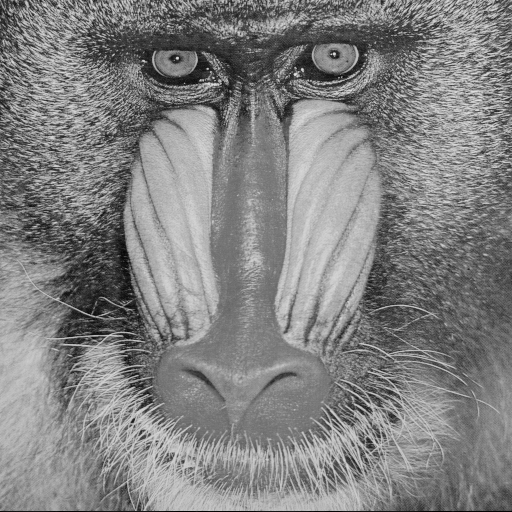
\includegraphics[width=5cm]{../out/baboon.png} }}%	
%	\caption{Imagens utilizadas para aplicação das técnicas de meios-tons por difusão de erro.}%	
%	\label{fig:imagem:entrada}%
%\end{figure}
%
%Para comparação com as imagens resultantes das técnicas de meios-tons por difusão de erro, gerou-se imagens denominadas controle a partir da aplicação da técnica de meio-tom que utiliza apenas o limiar de 128 para tomada de decisão se a um pixel será atribuído o valor zero (0) ou o valor (1). As imagens controle da imagem Baboon nas versões colorida e em escala de cinza são apresentadas na Figura \ref{fig:imagem:controle}.
%
%\begin{figure}[!htp]%
%	\centering
%	
%	\subfloat[\centering Imagem controle na versão colorida]{{ 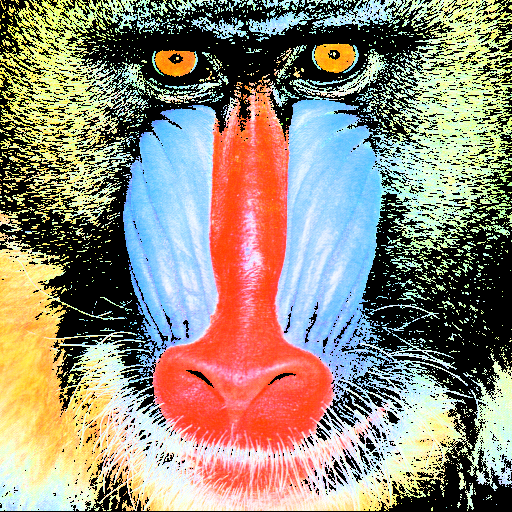
\includegraphics[width=5cm]{../out/cbaboon_control.png} }}%
%	\qquad
%	\subfloat[\centering Imagem controle na versão em preto e branco]{{ 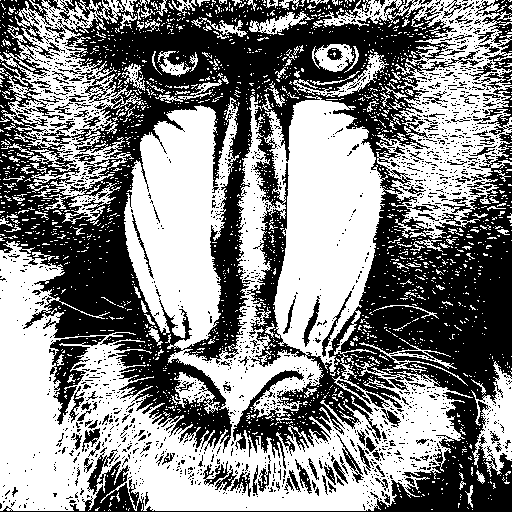
\includegraphics[width=5cm]{../out/baboon_control.png} }}%	
%	
%	\caption{Imagens controle para comparação com as imagens resultantes da aplicação da técnicas de meios-tons por difusão de erro.}%
%	
%	\label{fig:imagem:controle}%
%\end{figure}
%
%Na sequência, teremos a apresentação das imagens resultantes da aplicação das técnias de meios-tons por difusão de erro sobre a imagem Baboon na sua versão colorida e em escala de cinza.
%
%%
%\subsection{Técnicas de meios-tons sobre images em escala de cinza (varredura \textit{default})}
%Aqui serão apresentados as imagens resultantes da aplicação das técnicas de meios-tons sobre a imagem de entrada em escala de cinza.
%
%\begin{figure}[!htp]%
%	\centering
%	\subfloat[\centering Imagem em meio-tom pela técnica de Floyd e Steinberg]{{ 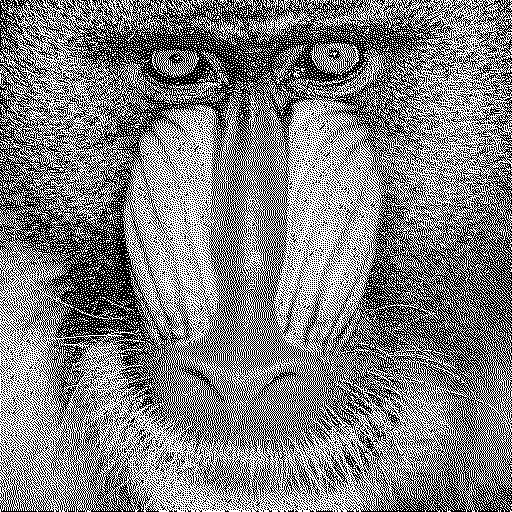
\includegraphics[width=3cm]{../out/baboon_floydsteinberg.png} }}%
%	\qquad
%    \subfloat[\centering Imagem em meio-tom pela técnica de Stevenson e Arce]{{ 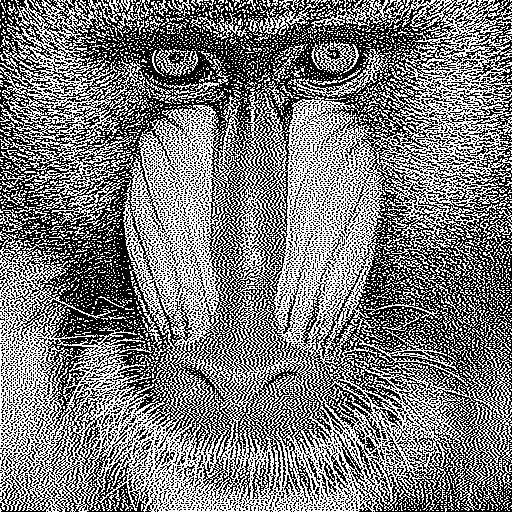
\includegraphics[width=3cm]{../out/baboon_stevensonarce.png} }}%
%	\qquad
%    \subfloat[\centering Imagem em meio-tom pela técnica de Burkers]{{ 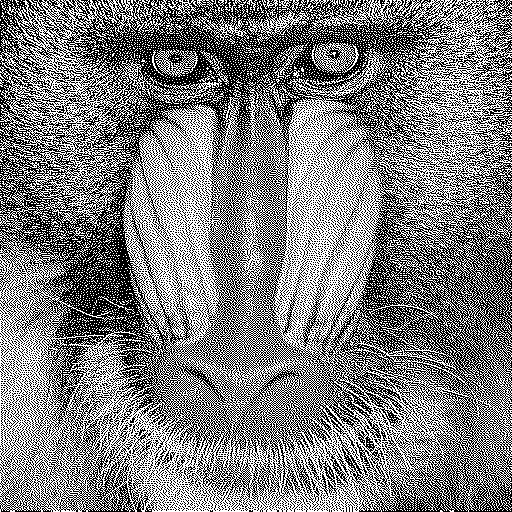
\includegraphics[width=3cm]{../out/baboon_burkers.png} }}%
%
%	\subfloat[\centering Imagem em meio-tom pela técnica de Sierra]{{ 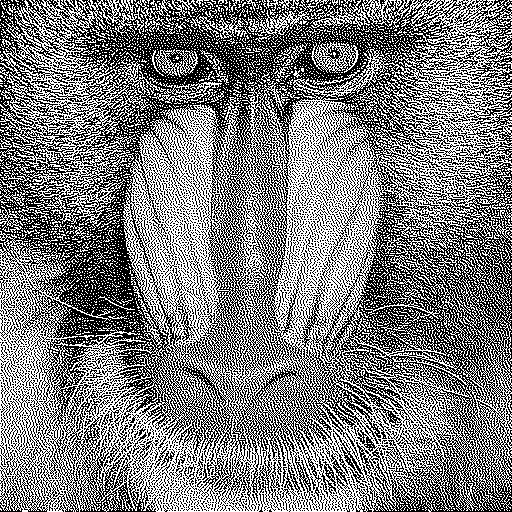
\includegraphics[width=3cm]{../out/baboon_sierra.png} }}%
%    \qquad
%   	\subfloat[\centering Imagem em meio-tom pela técnica de Stucki]{{ 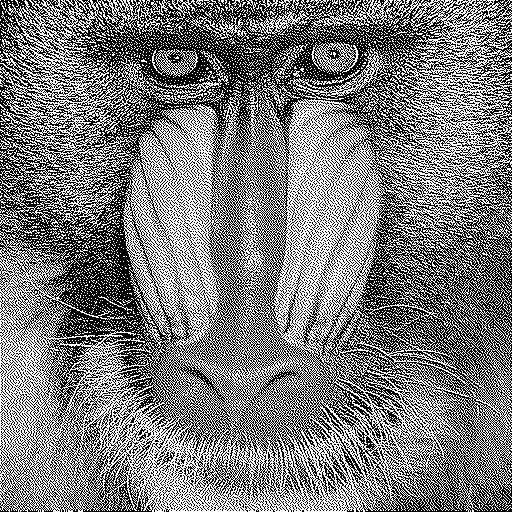
\includegraphics[width=3cm]{../out/baboon_stucki.png} }}%
%   	\quad
% 	\subfloat[\centering Imagem em meio-tom pela técnica de Javis, Judice e Ninke]{{ 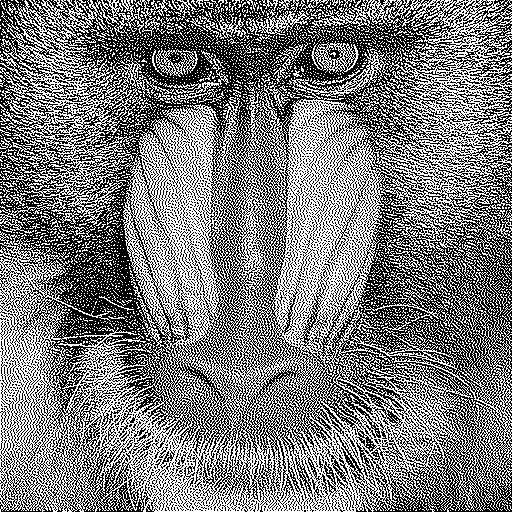
\includegraphics[width=3cm]{../out/baboon_jarvis.png} }}%
%	
%	\caption{Imagens resultantes em escala de cinza da aplicação das técnicas de meios-tons por difusão de erro em questão usando a varredura \textit{default}.}%
%	\label{fig:imagem:plano:baboon:cinza:1}%
%\end{figure}	
%
%%
%\subsection{Técnicas de meios-tons sobre images em escala de cinza (varredura zig-zag)}
%Aqui serão apresentados as imagens resultantes da aplicação das técnicas de meios-tons sobre a imagem de entrada em escala de cinza.
%
%\begin{figure}[!htp]%
%	\centering
%	\subfloat[\centering Imagem em meio-tom pela técnica de Floyd e Steinberg]{{ 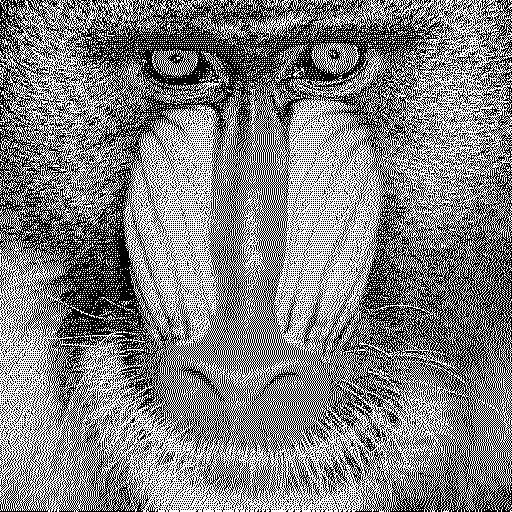
\includegraphics[width=3cm]{../out/zbaboon_floydsteinberg.png} }}%
%	\qquad
%	\subfloat[\centering Imagem em meio-tom pela técnica de Stevenson e Arce]{{ 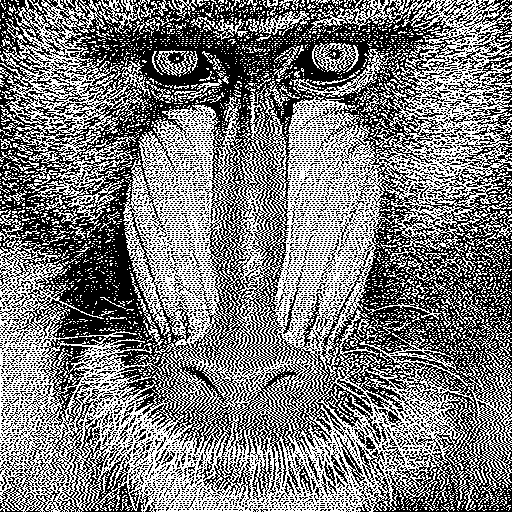
\includegraphics[width=3cm]{../out/zbaboon_stevensonarce.png} }}%
%	\qquad
%	\subfloat[\centering Imagem em meio-tom pela técnica de Burkers]{{ 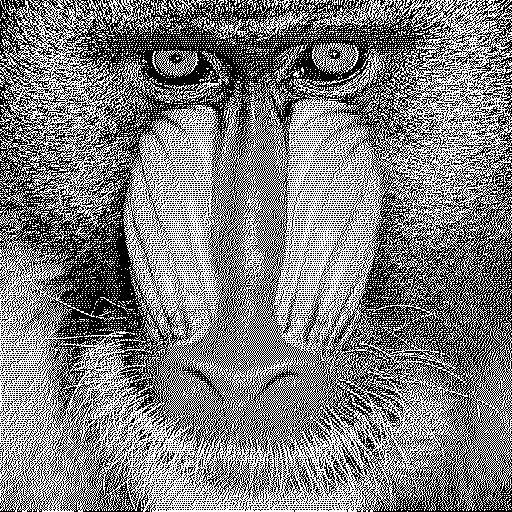
\includegraphics[width=3cm]{../out/zbaboon_burkers.png} }}%
%	
%	\subfloat[\centering Imagem em meio-tom pela técnica de Sierra]{{ 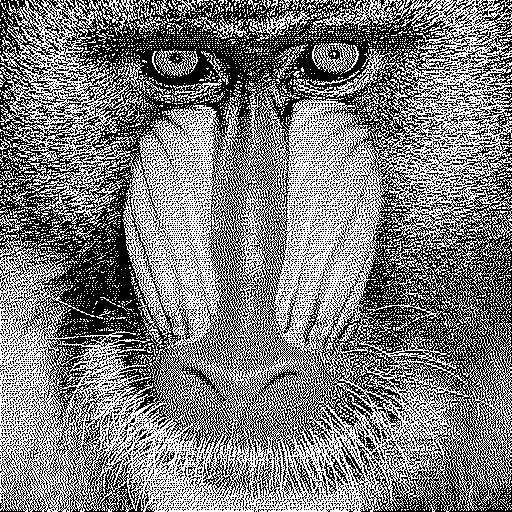
\includegraphics[width=3cm]{../out/zbaboon_sierra.png} }}%
%	\qquad
%	\subfloat[\centering Imagem em meio-tom pela técnica de Stucki]{{ 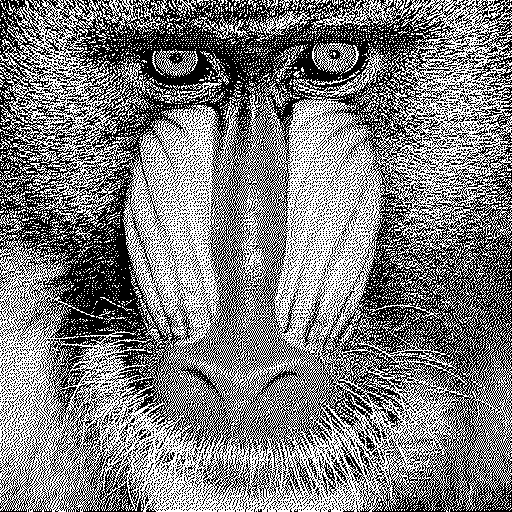
\includegraphics[width=3cm]{../out/zbaboon_stucki.png} }}%
%	\quad
%	\subfloat[\centering Imagem em meio-tom pela técnica de Javis, Judice e Ninke]{{ 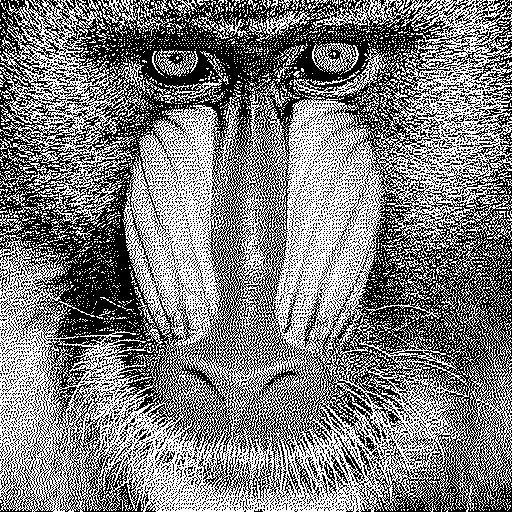
\includegraphics[width=3cm]{../out/zbaboon_jarvis.png} }}%
%	
%	\caption{Imagens resultantes em escala de cinza da aplicação das técnicas de meios-tons por difusão de erro em questão usando a varredura zig-zag.}%
%	\label{fig:imagem:plano:baboon:cinza:2}%
%\end{figure}	
%
%%
%\subsection{Técnicas de meios-tons sobre images coloridas (varredura \textit{default})}
%Temos a seguir apresentadas as imagens resultantes da aplicação das técnicas de meios-tons sobre a imagem de entrada colorida.
%
%\begin{figure}[!htp]%
%	\centering
%	\subfloat[\centering Imagem em meio-tom pela técnica de Floyd e Steinberg]{{ 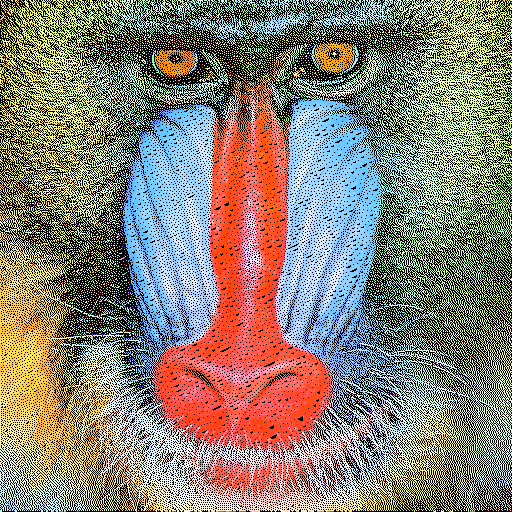
\includegraphics[width=3cm]{../out/cbaboon_floydsteinberg.png} }}%
%	\qquad
%	\subfloat[\centering Imagem em meio-tom pela técnica de Stevenson e Arce]{{ 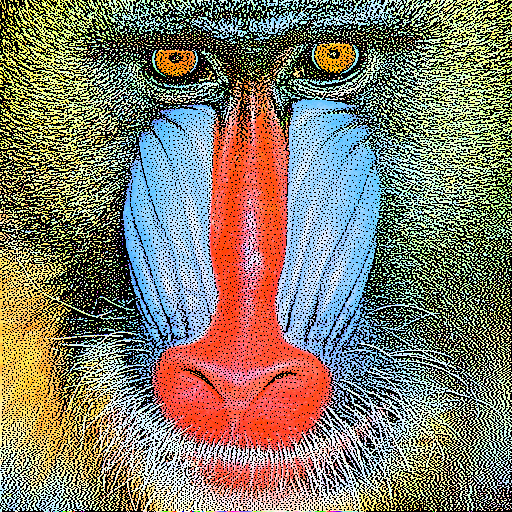
\includegraphics[width=3cm]{../out/cbaboon_stevensonarce.png} }}%
%	\qquad
%	\subfloat[\centering Imagem em meio-tom pela técnica de Burkers]{{ 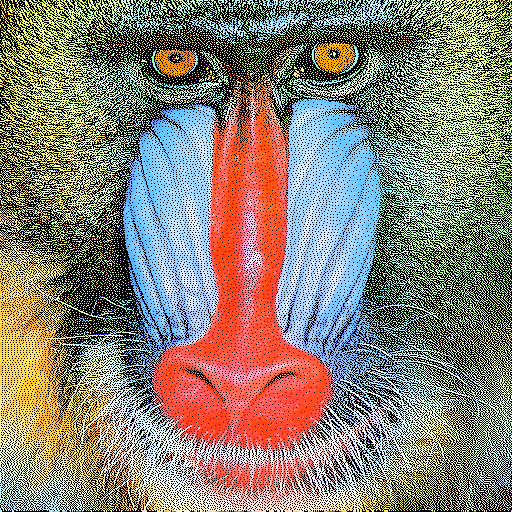
\includegraphics[width=3cm]{../out/cbaboon_burkers.png} }}%
%	
%	\subfloat[\centering Imagem em meio-tom pela técnica de Sierra]{{ 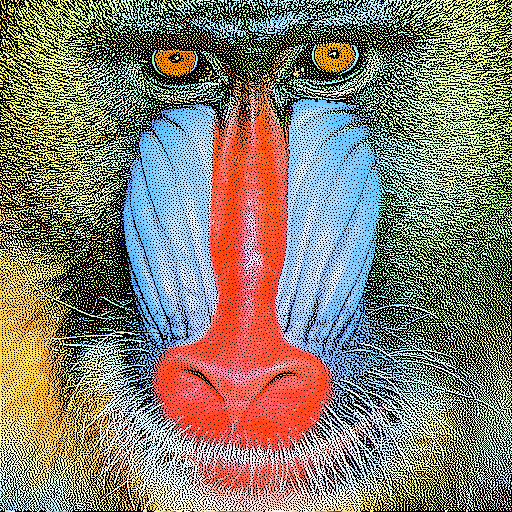
\includegraphics[width=3cm]{../out/cbaboon_sierra.png} }}%
%	\qquad
%	\subfloat[\centering Imagem em meio-tom pela técnica de Stucki]{{ 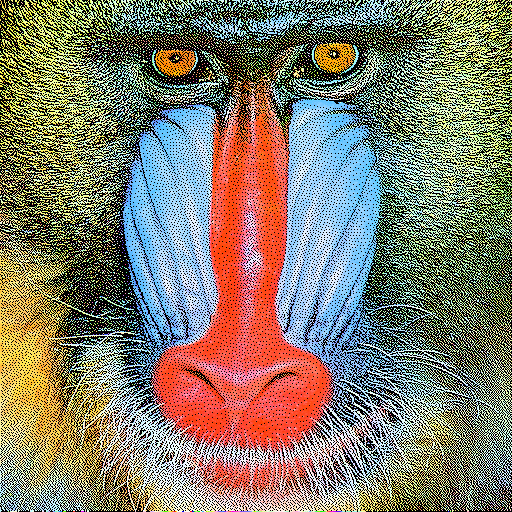
\includegraphics[width=3cm]{../out/cbaboon_stucki.png} }}%
%	\quad
%	\subfloat[\centering Imagem em meio-tom pela técnica de Javis, Judice e Ninke]{{ 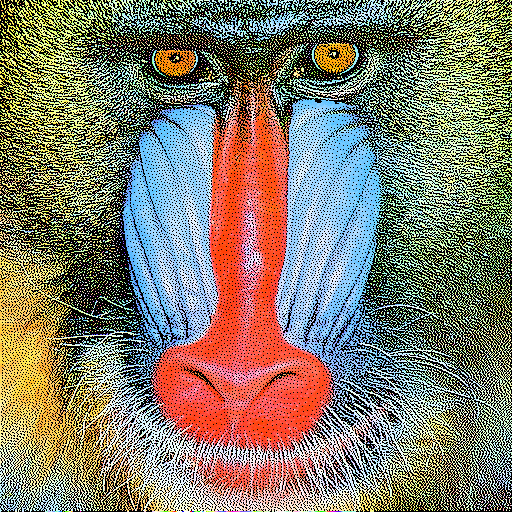
\includegraphics[width=3cm]{../out/cbaboon_jarvis.png} }}%
%	
%	\caption{Imagens resultantes coloridas da aplicação das técnicas de meios-tons por difusão de erro em questão usando a varredura \textit{default}.}%
%	\label{fig:imagem:plano:baboon:colorido:1}%
%\end{figure}
%
%
%%
%\subsection{Técnicas de meios-tons sobre images coloridas (varredura zig-zag)}
%Temos a seguir apresentadas as imagens resultantes da aplicação das técnicas de meios-tons sobre a imagem de entrada colorida.
%
%\begin{figure}[!htp]%
%	\centering
%	\subfloat[\centering Imagem em meio-tom pela técnica de Floyd e Steinberg]{{ 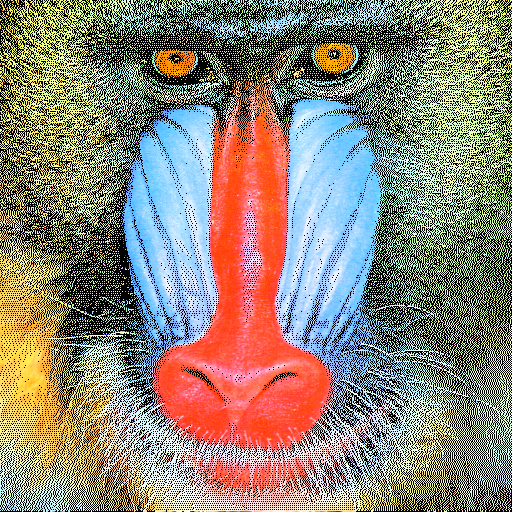
\includegraphics[width=3cm]{../out/czbaboon_floydsteinberg.png} }}%
%	\qquad
%	\subfloat[\centering Imagem em meio-tom pela técnica de Stevenson e Arce]{{ 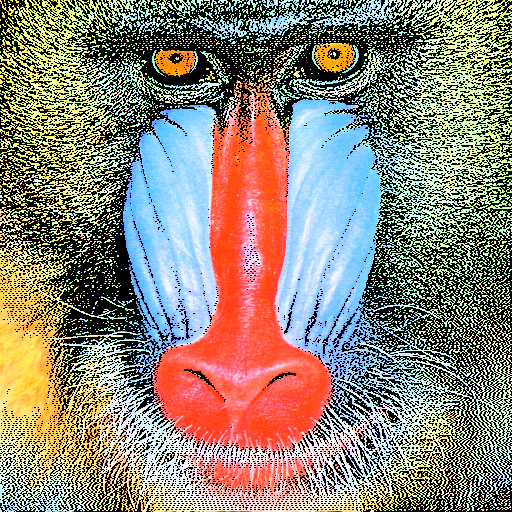
\includegraphics[width=3cm]{../out/czbaboon_stevensonarce.png} }}%
%	\qquad
%	\subfloat[\centering Imagem em meio-tom pela técnica de Burkers]{{ 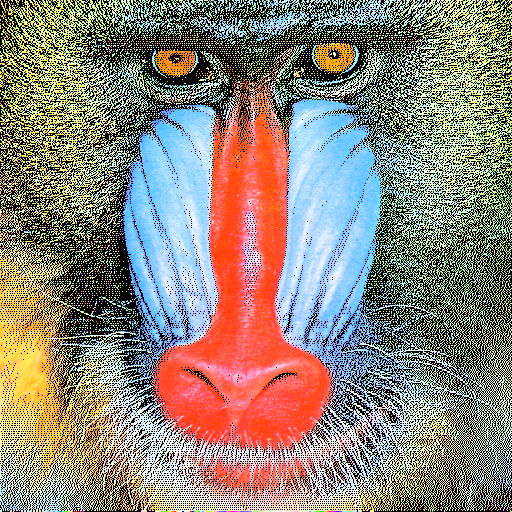
\includegraphics[width=3cm]{../out/czbaboon_burkers.png} }}%
%	
%	\subfloat[\centering Imagem em meio-tom pela técnica de Sierra]{{ 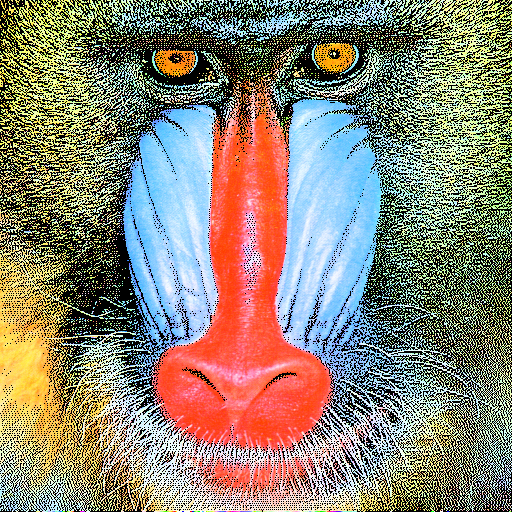
\includegraphics[width=3cm]{../out/czbaboon_sierra.png} }}%
%	\qquad
%	\subfloat[\centering Imagem em meio-tom pela técnica de Stucki]{{ 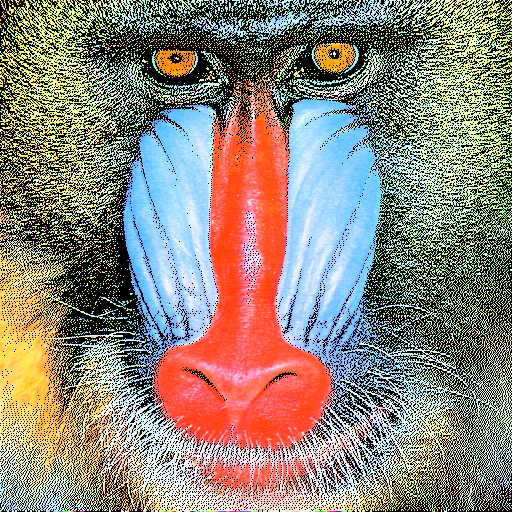
\includegraphics[width=3cm]{../out/czbaboon_stucki.png} }}%
%	\quad
%	\subfloat[\centering Imagem em meio-tom pela técnica de Javis, Judice e Ninke]{{ 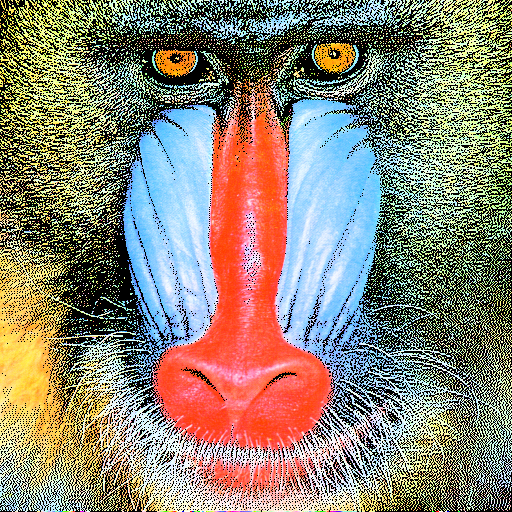
\includegraphics[width=3cm]{../out/czbaboon_jarvis.png} }}%
%	
%	\caption{Imagens resultantes coloridas da aplicação das técnicas de meios-tons por difusão de erro em questão usando a varredura zig-zag.}%
%	\label{fig:imagem:planocolorido:2}%
%\end{figure}
%
%\section{Dicussão e Conclusão}
%Do apresentado, podemos concluir que as técnicas de meios-tons foram aplicadas satisfatoriamente tanto sobre imagens coloridas quanto sobre imagens em escala de cinza. Para a imagem utilizada e dentro das dimensões consideradas, as ténicas de meios-tons tiveram resultados visuais semelhantes e bastante satisfatórios. Agora, dentro de uma análise mais minuciosa (ampliando-se as imagens) a técnica de meio-tom de Floyd e Steinberg apresentou uma imagem resultante com algumas falhas e vazios pretos na imagem resultante que não foram apresentados pelas imagens resultantes da aplicação das outras técnicas de meios-tons. Desse modo, quanto ao criterio visual, pode-se afirmar que a técnica de meio-tom de Floyd Steinberg apresentou os resultados menos interessantes com relação a harmonia visual da imagem resultante. Por outro lado, a aplicação da técnica de meio-tom de Floyd Steinberg é a menos custosa computacionalmente, dado que dispõe da menor mascara.
%
%Sobre as duas varreduras utilizadas, verifica-se que o resultante de ambas foi visualmente similar para a imagem utilizada. A diferença mais notável, foi que as imagens resultantes da aplicação das técnicas de meios-tons pela varredura em zig-zag ficaram com maior contraste que as imagens resultantes da varredura \textit{default}. Talvez para aplicações mais sofisticadas em que a qualidade das imagens em meios-tons seja crítica, a utilização de padrões de varredura mais complexos seja justificado, o que não é o caso dentro do contexto deste trabalho.
%
%%Do apresentado neste trabalho, podemos concluir que a esteganografia é uma técnica interessante e promissora de ocultação de mensagens em imagens sem que estas apresentem modificações visuais ao olho humano. De qualquer maneira, mesmo que visualmente as imagens não sejam alteradas, verificamos que ainda sim é possível identificar que a imagem está modifica e, assim, possivelmente com alguma mensagem escondida. Neste trabalho, essa verificação foi feita pela análise dos planos de bits das imagens modificadas. Nesse verificação, foi possível visualizar uma alteração do padrão de bits do plano de bits 0 (plano onde foi inserida a mensagem) em ambas as imagens Baboon e Watch utilizadas. A única exceção aconteceu com a imagem Baboon e a mensagem escondida \textbf{texto1.txt} que se deu, principalmente, porque a mensagem utilizada é muito pequena.


\end{document}
